\documentclass{article}

% if you need to pass options to natbib, use, e.g.:
% \PassOptionsToPackage{numbers, compress}{natbib}
% before loading nips_2018

% ready for submission
\usepackage{nips_2018}

% to compile a preprint version, e.g., for submission to arXiv, add
% add the [preprint] option:
% \usepackage[preprint]{nips_2018}

% to compile a camera-ready version, add the [final] option, e.g.:
% \usepackage[final]{nips_2018}

% to avoid loading the natbib package, add option nonatbib:
% \usepackage[nonatbib]{nips_2018}

\usepackage[utf8]{inputenc} % allow utf-8 input
\usepackage[usenames,dvipsnames]{color}
\usepackage[T1]{fontenc}    % use 8-bit T1 fonts
\usepackage{hyperref}       % hyperlinks
\usepackage{url}            % simple URL typesetting
\usepackage{booktabs}       % professional-quality tables
\usepackage{amsmath}
\usepackage{amssymb}
\usepackage{amsfonts}       % blackboard math symbols
\usepackage{nicefrac}       % compact symbols for 1/2, etc.
\usepackage{microtype}      % microtypography
\usepackage[pdftex]{graphicx} 

\usepackage{algorithm}
\usepackage{algorithmic}
% Attempt to make hyperref and algorithmic work together better:
%\newcommand{\theHalgorithm}{\arabic{algorithm}}

\title{Visual scene decoding through fovea-based computation} %: a variational perspective}
%\title{Predictive information maximizing control: a unifying view}
% The \author macro works with any number of authors. There are two
% commands used to separate the names and addresses of multiple
% authors: \And and \AND.
%
% Using \And between authors leaves it to LaTeX to determine where to
% break the lines. Using \AND forces a line break at that point. So,
% if LaTeX puts 3 of 4 authors names on the first line, and the last
% on the second line, try using \AND instead of \And before the third
% author name.

\author{
  Emmanuel Daucé\\
  Ecole Centrale de Marseille,\\ 
  Aix Marseille Univ, Inserm,\\ 
  INS, Institut de Neurosciences des Systèmes, \\
  Marseille, France\\
  \texttt{emmanuel.dauce@centrale-marseille.fr} 
}

\begin{document}
% \nipsfinalcopy is no longer used

\maketitle

\begin{abstract}
Large images are annoying for they own lot of pointless and repetitive features that should be bypassed
when the computing resources are at stake. Efficient scene analysis thus supposes to optimize the choice of the 
pixels that will be decoded to achieve a certain task. We consider here the case of sequential \emph{fovea-based} image decoding, which 
is a multi-scale focal sensing principle inspired by animal vision. The images are analyzed  
through moving an artificial \emph{center of sight}, that grabs information in small parts of the total scene 
to perform recognition. 
This sequential approach to visual scene decoding is presented and optimized under 
information-theoretic first principles, issuing an efficient decoding setup that shows (i) 
state-of-the-art recognition rate when less than 10\% of the original signals is used, (ii) a good up-scaling capability 
and (iii) a near-optimal robustness to model flaws, that overtakes the many concurrent methods 
used in literature.
\end{abstract}

\section{Motivation}

Though ubiquitous in biology, object recognition through saccades is seldom considered in artificial vision. One reason is the existence of highly effective sensors, providing millions of pixels at low cost. Increasingly powerful parallel devices are then assigned to compute those pixels to perform recognition, consuming resources in a brute-force fashion. 
The example of animal vision encourages however a different approach towards more parsimonious recognition algorithms. A salient aspect of animal vision is indeed the use of \emph{active} sensing devices, with variable center-surround resolution, that move around within some degrees of freedom in order to choose a particular viewpoint. The important redundancy present in the visual data was exploited by natural selection,  ending up in energy-efficient visual exploration policies, exploiting only little portions of the visual environment to decode the total sensory scene.
Though the opportunity to neglect large parts of the visual scene is generally considered when the energy is scarce, as it is the case for drones and robots, 
%that need to react fast with light and low-power sensing devices. 
high resolution images appeal for \emph{selective processing} over large pixel fields. 
%A computer vision program should for instance look back from past experience to see which viewpoint to use to provide the most useful information about a scene. 
%Selecting the relevant pixels across time may then be a part of computer vision algorithms, in combination with traditional convolution-based computations. 
%The idea of viewpoints selection turns out to consider beforehand the pixels that need to be processed to achieve the scene decoding. 
%The general principle is that of
%choosing the viewpoint that is the most {\color{blue} informative} \emph{in expectation}. 
%This entails \emph{predicting the future information gain} made by choosing a given viewpoint over the total scene. 
Two parallel research tracks adopted and refined this very idea over the last twenty years. A first track, developed in robotics and control, insists on the formal contribution of action in encoding the sensory field. This resorts to consider action as a \emph{code} that is later on revealed (decoded) by sensing the effect of action at the visual field \citep{klyubin2005empowerment,tishby2011information}. As such it may be optimized so as to maximize the code effectiveness, allowing to improve both the policy and the data model in the course of learning \citep{schmidhuber2007simple,mohamed2015variational,houthooft2016vime}. Another line of research, initially developed in human visual search modeling, considers action as a \emph{sampling} an underlying (covert) sensory scene. Then appropriate samples should be selected to maximize the \emph{decoding accuracy}, that resorts to refine the beliefs about the underlying scene to reduce the posterior entropy (see \cite{najemnik2005optimal,najemnik2009simple,butko2010infomax,friston2012perceptions}).
We provide here a way to reconcile the two views when considering action as being both a code and a sampling. 
%This is done through postulating a bijection between the motor command and the actuator state.
In our setup, the current observation is the decoding of a \emph{mixed code}  
made of a controlled code (i.e. the actuator state) and an uncontrolled one (i.e. the rest of the environment). This idea is first mathematically developed in section \ref{sec:principles}, providing a way to unify the different objective functions found in the literature. 
Then a fovea-based implementation is proposed in section \ref{sec:fovea}, allowing to compare in detail the different options in a single setup, and propose new avenues toward more parsimonious scene decoding through computationally-effective model-based prediction.

%Less intuitively, the ever-growing  learning databases used in machine learning also suggest an intelligent scanning of the data, in a way that should retain only the critical examples or features, depending on the context, before performing learning on it.  
%Behind the viewpoint selection problem thus lies a feature selection problem, which should rely on a context. 
 \section{Principles}\label{sec:principles}
We consider here a \emph{scene decoding task} where an agent has to estimate its environment state, here called the ``sensory scene'' from sensory samples. The visual scene is organized in objects (or objects parts), whose presence and position is continuously checked by visual inspection. 
Then, decoding a visual scene through saccades consists in identifying the ensemble through the foveation of parts of the scene only. 
We here suppose that a generative model $p$ is given to the agent, that is a probability distribution over $\boldsymbol{z} \in \mathcal{Z}$ (the scene encoding),  $\boldsymbol{u} \in \mathcal{U}$ (the current viewpoint) and $\boldsymbol{x} \in \mathcal{X}$ (the current view), i.e. $\boldsymbol{x}, \boldsymbol{z}, \boldsymbol{u} \sim p(X,Z,U)$.
%Stemming from a general POMDP standpoint, important simplifications are considered here, namely (i) \emph{Emitters independence}, that is $p(\boldsymbol{z}, \boldsymbol{u}) = p(\boldsymbol{z})p(\boldsymbol{u})$ so that
%any scene can be observed from any viewpoint; 
%\emph{(ii) End-effector control}, 
%that is the controlled generative process is relatively ``fast'' in comparison with the uncontrolled one
%(for, e.g, saccades can be realized in a 100-200 ms interval). 
%In consequence the motor command  $\boldsymbol{u}$ is considered as a setpoint (or posture) in the actuator space, that is supposed to be reached 
%at short notice once the command is emitted, under classical stability/controllability constraints; \emph{(iii) Uncontrolled environment}, that is the motor command $\boldsymbol{u}$ \emph{is not expected to affect the  latent state $\boldsymbol{z}$},
%so that $\boldsymbol{z}$ should depend only on the external dynamics (the external ``uncontrolled'' process); and
%\emph{(iv) Static assumption}
%i.e. the scene is not changing over time \cite{butko2010infomax}. 
%The uncontrolled latent emitter $\boldsymbol{z}$ is thus expected to capture all relevant information about the current scene, while remaining invariant throughout the decoding process.
Each different viewpoint $\boldsymbol{u}$ drives a different sensory fields over the same underlying sensory scene, and $\boldsymbol{x}$ (the view) and $\boldsymbol{z}$ (the \emph{latent state}) are now the realization of a generative model parametrized by $\boldsymbol{u}$, i.e.
\begin{align}
\boldsymbol{x}, \boldsymbol{z} | \boldsymbol{u} \sim p(X|Z, \boldsymbol{u}), p(Z)
\end{align}  
Each measure $\boldsymbol{x}$ is generated from a mixed code $(\boldsymbol{z}, \boldsymbol{u})$, with $\boldsymbol{u}$ the controlled part of the code and  $\boldsymbol{z}$ the uncontrolled part. %, so that $p(X,Z,U) = p(X|Z, U) p(X, U)$. 
Note that $\boldsymbol{z}$ is said the latent state out of habit, though both $\boldsymbol{u}$ and $\boldsymbol{z}$ contribute to the generation of $\boldsymbol{x}$.

\paragraph{Variational scene encoding}\label{sec:encoding}
%In a model-based approach, the latent variable $\boldsymbol{z}$ is expected to specify the state of the physical environment. In the model-free case, only weak assumptions need to be made about the latent space.  The latent space $\mathcal{Z}$ just needs to be expressive enough to capture and restore all necessary information about the environment.  
The \emph{variational encoding} perspective  was originally developed 
to train unsupervised autoencoder neural networks \citep{hinton2006reducing}. 
%The general idea is that an efficient code 
%is a code that is both compact and accurate at restoring the data. 
If $\boldsymbol{x}$ is the original data, the corresponding code $\boldsymbol{z}$ is generated by a distribution $q$, i.e. $\boldsymbol{z} \sim q(Z)$. This distribution is called the \emph{encoder}. Then, the reconstruction is rendered possible with a second conditional probability over the codes, i.e. $p(X|\boldsymbol{z})$, that is called the \emph{decoder}. 
%If $\boldsymbol{z}$ is the current code, the reconstructed data is $\tilde{\boldsymbol{x}} \sim p(X|\boldsymbol{z})$. 
%Then, t
The efficacy of a code is estimated by an information-theoretic quantity, the ``reconstruction cost'' \citep{hinton1994autoencoders} that is defined for every $\boldsymbol{x}$ knowing $p$ and $q$.
In our case, the reconstruction cost writes:
\begin{align}
F(\boldsymbol{x}|\boldsymbol{u}) 
&= \mathbb{E}_{z\sim q} \left[-\log (p(\boldsymbol{x}|\boldsymbol{z},\boldsymbol{u})p(\boldsymbol{z}))\right] - H(q)\\
&= \mathbb{E}_{z\sim q} \left[-\log (p(\boldsymbol{x}|\boldsymbol{z},\boldsymbol{u}))\right] +\text{KL}(q(Z)||p(Z))
\label{eq:FEP-prior-u}\\
&= - \log p(\boldsymbol{x}|\boldsymbol{u}) + \text{KL}(q(Z)||p(Z|\boldsymbol{x}, \boldsymbol{u}))
\label{eq:FEP-posterior-u}\end{align}
%\begin{align}
%F(\boldsymbol{x};p,q) = - \sum_{\boldsymbol{z} \in \mathcal{Z}} q(\boldsymbol{z}) \log (p(\boldsymbol{x}|\boldsymbol{z})p(\boldsymbol{z})) - H(q)
%= \mathbb{E}_{z\sim q} \left[-\log (p(\boldsymbol{x}|\boldsymbol{z})p(\boldsymbol{z}))\right] - H(q)
%\label{eq:FEP-energy}
%\end{align}
%with $\mathcal{Z}$ an arbitrary encoding space, $q$ an arbitrary distribution over the codes, $H(q) = -\sum_z q(\boldsymbol{z}) \log q(\boldsymbol{z})$ the entropy of $q$, $p(X|Z)$ the decoder and $p(Z)$ a prior distribution over the codes.
The densities $p$ and $q$ are called ``variational'' for they can be optimized according to the data \citep{hinton2006fast,kingma2013auto}.  
%$F$ is also called the variational Free Energy for it is mathematically analog to the Helmhotz Free Energy.
It is shown in \cite{kingma2013auto} that an optimal code $q(Z)\simeq p(Z|\boldsymbol{x})$ can be approached through a stochastic gradient descent over $p$ and $q$ according to $-\nabla_{p,q} F(\boldsymbol{x}) $	so that the reconstruction cost should meet the ``description length'' of the data \citep{hinton1994autoencoders}, i.e. its estimated (natural) Shannon Information under the model $p$.

%If we now turn back to the viewpoint selection setup, an additional factor $\boldsymbol{u}$ (the viewpoint) comes into the play. The data $\boldsymbol{x}$ that is actually read is now conditioned on  $\boldsymbol{u}$, so that
%with each viewpoint $\boldsymbol{u}$ providing a distinct optimization problem. 

\paragraph{Sequential Bayesian inference}

The chaining of the posterior to the role of the prior in the next inference step is a classical property of sequential Bayesian inference \citep{wald1945sequential}.
When generalized to many observations: $(\boldsymbol{x},\boldsymbol{u}), (\boldsymbol{x}',\boldsymbol{u}')$, ..., $(\boldsymbol{x}^{(n)},\boldsymbol{u}^{(n)})$, the final code $q^{(n)}(Z)$ writes:
\begin{align}
q^{(n)}(Z) \propto p(\boldsymbol{x}|Z,\boldsymbol{u}) p(\boldsymbol{x}'|Z,\boldsymbol{u}') ... p(\boldsymbol{x}^{(n)}|Z,\boldsymbol{u}^{(n)}) \label{eq:accum}
\end{align}
It is noteworthy that the $\boldsymbol{u}$'s and $\boldsymbol{x}$'s do not need to be stored in the process. At step $n$, only $q^{(n-1)}$ (the current ``belief'') needs to be memorized to estimate $q^{(n)}$, i.e. 
\begin{align} 
q^{(n)}(Z) \propto p(\boldsymbol{x}^{(n)}|Z,\boldsymbol{u}^{(n)}) \times q^{(n-1)}(Z) \label{eq:accum-post}
\end{align}
Finally, from the encoding point of view, the $n^\text{th}$ reconstruction cost $F^{(n)}(\boldsymbol{x}^{(n)}|\boldsymbol{u}^{(n)}, ..., \boldsymbol{x}, \boldsymbol{u})$ also obeys to the chain rule, i.e. is estimated from $q^{(n-1)}$, $\boldsymbol{u}^{(n)}$ and $\boldsymbol{x}^{(n)}$ only:
\begin{align}
F(\boldsymbol{x}^{(n)}|\boldsymbol{u}^{(n)}; q^{(n)}) 
&= \mathbb{E}_{\boldsymbol{z} \sim q^{(n)}} \left[-\log p(\boldsymbol{x}^{(n)}| \boldsymbol{u}^{(n)}, \boldsymbol{z})\right] + \text{KL}(q^{(n)}(Z)||q^{(n-1)}(Z))
\label{eq:FEP-uxun}
\end{align}
%The posterior of a prior step has been passed to the next estimation step and now plays the role of the prior.  This shows that a single distribution $q_\text{\sc post}(Z_{t-1})$ needs to be conserved in memory to calculate the next estimate $q_\text{\sc post}(Z_t)$, i.e.:
with $q^{(n)}$ the shared (or cumulative) code according to the past and current observations, with $q^{(n-1)}$ having the role of the prior, providing a \emph{forward} variational encoding scheme (see also \cite{fraccaro2016sequential} for a backward implementation). 

\paragraph{Existing work}
Considering now the \emph{scene decoding task}, 
%where an agent has to estimate its environment state $\boldsymbol{z}$ from sampling it from different viewpoints. We here suppose that a generative model  is given to the agent. 
%Depending on  the current viewpoint $\boldsymbol{u}$, a different view $\boldsymbol{x}$ is observed at the sensors. So, each different command $\boldsymbol{u}$ provokes a different observation, and thus a different 
%estimation of the latent state. It is thus worth to question what is the optimal choice for $\boldsymbol{u}$ in order to maximize the accuracy of the posterior estimate?
%That turns  to minimize the number of samples so as to provide an accurate estimate. This approach to inference is called \emph{active sampling} \cite{friston2012perceptions}, for the choice of $\boldsymbol{u}$ determines the sensory sample $\boldsymbol{x}$ that is observed, conditioning the final posterior estimate.
a baseline sampling strategy is to choose $\boldsymbol{u}^{(n)}$ at random and condition the posterior  estimate on this random action. 
More elaborate strategies consider the past observations
%$\{\boldsymbol{u}^{(1:n-1)}, \boldsymbol{x}^{(1:n-1)}\}$ 
to choose the most promising action $\hat{\boldsymbol{u}}$. %We have seen in  \ref{sec:perception-driven-control} that, under a Markov assumption, the memory of the past context
%at step $n$ .  
The knowledge about past observations being here absorbed in single posterior distribution $q^{(n-1)}$, the problem turns out to design  a \emph{controller} $C$ which, given a context $q^{(n-1)}$, sets up an action $\hat{\boldsymbol{u}} = C(q^{(n-1)})$. 
%Here the role of the controller is not to achieve a goal-oriented task, but to render the estimation of the latent state more accurate. The controller is said \emph{perception-driven}. 
%The design of such a controller is not straightforward. 
%On contrary to classical control, there is not definite setpoint $\boldsymbol{z}^*$ to which the controller is supposed to drive the external process (through model inversion for instance). 

The predictive approach to perception-driven control was originally developed by \cite{najemnik2005optimal} to the case of visual search.
The predictive approach relies on predicting an \emph{objective} function $A(\boldsymbol{x}, \boldsymbol{u}, q^{(n-1)})$ to choose action, that may tell how good the model is at predicting $\boldsymbol{z}$  when viewing $\boldsymbol{x}$ at position $\boldsymbol{u}$,
knowing $q^{(n-1)}$.
The optimal action at time $n$ is:
\begin{align}
\hat{\boldsymbol{u}} = \underset{\boldsymbol{u} \in \mathcal{U}}{\text{ argmax }} \bar{A}(\boldsymbol{u}, q^{(n-1)})
\label{eq:predictive-policy}
\end{align}
with $\bar{A}(\boldsymbol{u}, q^{(n-1)})
= \mathbb{E}_{\boldsymbol{z} \sim q^{(n-1)}(Z), \boldsymbol{x} \sim p(X|\boldsymbol{z}, \boldsymbol{u})}\left[A(\boldsymbol{x}, \boldsymbol{u}, q^{(n-1)})\right]$ the \emph{predicted} objective attached to $\boldsymbol{u}$, 
formally similar to the Value in Reinforcement Learning (i.e. estimate of a future objective)\footnote{It must be noted that in order to render the computations tractable, a sampling approach is generally used to estimate the predicted accuracy, i.e. $\mathbb{E}_p[f(\boldsymbol{x})] \simeq f(\tilde{\boldsymbol{x}})$, with $\tilde{\boldsymbol{x}}\sim p(\boldsymbol{x})$.}.
Many such objective functions are proposed in the literature. They are generally referred as an \emph{intrinsic} motivation \cite{oudeyer2008can} by contrast with the \emph{extrinsic} motivation that relates to the classical rewards in Reinforcement Learning \cite{sutton1998reinforcement}.
The accuracy measure used in the original paper was an ad-hoc one \cite{najemnik2005optimal}, but turned out to be consistent with minimizing the \emph{posterior entropy} \cite{najemnik2009simple}, i.e.:
$A(\boldsymbol{x}, \boldsymbol{u}, q^{(n-1)}) = -H(q^{(n)}) = \sum_{z \in \mathcal{Z}} q^{(n)}(\boldsymbol{z}) \log q^{(n)}(\boldsymbol{z})$. This approach to optimal visual sampling was further on linked to an ``Infomax'' principle in \cite{butko2010infomax} 
%and shown efficient in artificial visual search using policy gradient \cite{williams1992simple} to learn the controller, with 
taking
\begin{align}A(\boldsymbol{x}, \boldsymbol{u}, q^{(n-1)}) \equiv I(Z; \boldsymbol{x}|\boldsymbol{u}, q^{(n-1)})
= H(Z|q^{(n-1)}) - H(Z|\boldsymbol{x}, \boldsymbol{u}, q^{(n-1)})
\label{eq:infomax}
\end{align}
with  $H(Z|X, \boldsymbol{u}, q^{(n-1)}) \equiv H(q^{(n)})$.
The Infomax (or posterior entropy minimization) approach generally makes sense for it implicitly relies on the chaining from $q^{(n-1)}$ to $q^{(n)}$, that considers that if $p(\boldsymbol{x}|Z, \boldsymbol{u})$ is consistent with $q^{(n-1)}(Z)$, then the issued posterior entropy should be lower than if $p(\boldsymbol{x}|Z, \boldsymbol{u})$ is at odd with $q^{(n-1)}(Z)$. The model is expected to choose the action that may confirm the initial assumption, though there is no cross-entropy comparison between $q^{(n-1)}$ and $q^{(n)}$.
It is thus potentially vulnerable to model outliers with $q^{(n)}$ having both a low entropy and being inconsistent with $q^{(n-1)}$. 


Another quantity of interest is the so-called \emph{Bayesian surprise} (or \emph{ Salience}) \citep{itti2005bayesian},
% defined as the Kullback-Leibler divergence {\color{blue} between an actual view $(\boldsymbol{x}, \boldsymbol{u})$ and a model $q^{(n-1)}$}.  
%In the original ``bottom-up'' setup, only local statistics $q$ are formed over small image patches of a given image, with $\boldsymbol{u}$ the index of a patch and $q(\boldsymbol{z}|\boldsymbol{x},\boldsymbol{u})$ the features inferred from the data actually observed at $\boldsymbol{u}$. For each patch $\boldsymbol{u}$, the \emph{salience} (or ``\emph{Bayesian surprise}'') of the actual view $\boldsymbol{x}$ given the model is:
%$$ S(\boldsymbol{x},\boldsymbol{u}) = \text{KL}(q(Z| \boldsymbol{x}, \boldsymbol{u})||q(Z))$$
which is a measure of the \emph{in}consistency between a (viewpoint independent)  model $q$ and the data $(\boldsymbol{x}, \boldsymbol{u})$. 
In our sequential setup, the salience writes:
\begin{align}
A(\boldsymbol{x}, \boldsymbol{u}, q^{(n-1)}) \equiv S(\boldsymbol{x},\boldsymbol{u}, q^{(n-1)}) = \text{KL}(q^{(n)}||q^{(n-1)})
\label{eq:saliency}
\end{align}
%A high salience reports a strong inconsistency with the model ({\color{blue} a high Bayesian surprise}), while a low salience reports a strong consistency with the model ({\color{blue} a low Bayesian surprise}).
%Here, consistent with the PEC alone, 
%with $q^{(n-1)}$ considered as the data model and $q^{(n)}$ the posterior estimated at $(\boldsymbol{x},\boldsymbol{u})$.
%It interestingly shares a formal similarity with the second term of the variational Free Energy (see eq.\ref{eq:FEP-uxun}). 
According to Itti and Baldi, the regions that have a high Bayesian surprise are the ones that attract the sight the most, so that, in a predictive setup, the predicted salience is to be \emph{maximized}.
%The calculation of $S(\boldsymbol{x}, \boldsymbol{z}| \boldsymbol{u})$ at each location $\boldsymbol{u}$ forms a \emph{saliency map} that is then considered as a prediction of where the sight will most likely be attracted (high values most probably attract the sight, low values less probably do). 
%In a sequential setup, a corresponding predictive policy would be:
%$$ \hat{\boldsymbol{u}} = \underset{\boldsymbol{u} \in \mathcal{U}}{\text{ argmax }} \mathbb{E}_{\boldsymbol{z} \sim q^{(n-1)}(Z), \boldsymbol{x} \sim p(X|\boldsymbol{z}, \boldsymbol{u})}\left[\text{KL}(q^{(n)}(Z)||q^{(n-1)}(Z))\right]$$
The saliency model has a strong explanatory power and provides among the best fit with the preferred fixation zones observed in humans.
Its scalability moreover provides straightforward applications in image and video compression  \cite{wang2003foveation,guo2010novel}.
%It  however constitutes a challenge to modelers, for it is at odd with scene interpretation,  
%It thus provides little explanation about the sight-orientation cognitive operations. 
%It is for instance known from eye-tracking data that humans sight is attracted by ``high-level'' features like faces, text or letters \cite{judd2009learning}, that are not captured by the low-level approach. 
%i.e. enters in contradiction 
%(or in ``dialectic'' contrast) 
%with the scene encoding setup, where one objective of the encoder is to minimize the divergence between the inferred code and the prior expectations (see \cite{friston2015active} for a discussion).

At last, the  active inference setup \citep{friston2010free,friston2012perceptions} 
considers the general tendency of the brain to counteract surprising and unpredictable sensory events through minimizing the Free Energy with action, that is  interpreted here as maximizing the ELBO\footnote{Evidence Lower BOund.} through action~:
\begin{align}
A(\boldsymbol{x}, \boldsymbol{u}, q^{(n-1)}) \equiv -F(\boldsymbol{x}|\boldsymbol{u}; q^{(n-1)}) = 
\log p(\boldsymbol{x}| \boldsymbol{u}; q^{(n-1)}) - \text{KL}(q^{(n-1)}||q^{(n)})
\label{eq:ELBO}
\end{align}
with $\text{KL}(q^{(n-1)}||q^{(n)})$ representing the interpretative effort made by interpreting  $\boldsymbol{x}|\boldsymbol{u}$ with $q^{(n)}$ instead of $q^{(n-1)}$. Minimizing $\text{KL}(q^{(n-1)}||q^{(n)})$ thus corresponds to a \emph{conservative} approach to the scene interpretation
that is \emph{minimally} vulnerable to outliers, i.e. that minimizes the risk of a false interpretation. It is obvious here that the ELBO and the Saliency are antithetic objectives, and no consensus is currently observed in literature about which objective should prevail (though Infomax generally preferred in scene decoding and saliency/surprise preferred in sparse reinforcement learning).

\paragraph{Shared code and information gain}
Following the intuition of \cite{friston2012perceptions}, the scene decoding setup shares a common formalism with the variational encoding setup, at the difference the changing of $F$ now relies on updating the observation set
with a new sample $(\boldsymbol{x}^{(n)}, \boldsymbol{u}^{(n)})$ rather than updating the model parameters.
%The structure of the problem (many views on the same scene) implies that the different  views should share a common \emph{information} corresponding to the actual (covered) sensory scene. 
The sharing of information between two sensory fields $(X, \boldsymbol{u})$ and $(X', \boldsymbol{u}')$ can be quantified by their \emph{mutual information}:
\begin{align}
I((X| \boldsymbol{u}); (X'| \boldsymbol{u}')) = H(X| \boldsymbol{u}) - H(X| \boldsymbol{u}', X', \boldsymbol{u})
= \mathbb{E}_{X,X'} \left[-\log p(X| \boldsymbol{u}) + \log p(X| \boldsymbol{u}', X', \boldsymbol{u})\right] \nonumber
%&\simeq \mathbb{E}_{X,X'} \left[F(X|\boldsymbol{u}) - F(X'|\boldsymbol{u}', X, \boldsymbol{u})\right] \label{eq:infomax}
\end{align}
with 
($i$) $ p(\boldsymbol{x}| \boldsymbol{u}', \boldsymbol{x}', \boldsymbol{u}) \triangleq \sum_{\boldsymbol{z}} p(\boldsymbol{x}|\boldsymbol{z}, \boldsymbol{u}) p(\boldsymbol{z}|\boldsymbol{x}', \boldsymbol{u}')$ 
the \emph{mutual} likelihood, i.e. the updated likelihood of $\boldsymbol{x}$ at $\boldsymbol{u}$ after seeing $\boldsymbol{x}'$ at $\boldsymbol{u}'$,
%($ii$) $-\log p(\boldsymbol{x}'| \boldsymbol{u}', \boldsymbol{x}, \boldsymbol{u})$
%the \emph{post-sample} approximate natural Shannon Information, 
and ($ii$) 
$-\log p(\boldsymbol{x}| \boldsymbol{u}) + \log p(\boldsymbol{x}| \boldsymbol{u}', \boldsymbol{x}', \boldsymbol{u})$ the 
\emph{information gain} \citep{tishby2011information}.
%We call it here the \emph{conditional Free Energy} (for it is conditioned over $\boldsymbol{x}, \boldsymbol{u}$)
%with: % the post-sample Shannon Information approached by the post-sample Free Energy as: 
An approximation of the information gain, known as the \emph{Compression Improvement} or CI \citep{schmidhuber2007simple,houthooft2016vime}
writes~:
\begin{align}
\text{CI}(\boldsymbol{x},\boldsymbol{u}, \boldsymbol{x}', \boldsymbol{u}') = F(\boldsymbol{x}|\boldsymbol{u};p,q) - F(\boldsymbol{x}|\boldsymbol{u}, \boldsymbol{x}', \boldsymbol{u}';p,q') 
\end{align}	
with $F(\boldsymbol{x}|\boldsymbol{u};p,q)$ the pre-sample cost and  
\begin{align}
F(\boldsymbol{x}|\boldsymbol{u}, \boldsymbol{x}', \boldsymbol{u}';p,q') &= 
\mathbb{E}_{z\sim q'} \left[-\log (p(\boldsymbol{x}|\boldsymbol{z}, \boldsymbol{u}) p(\boldsymbol{z}|\boldsymbol{x}', \boldsymbol{u}'))\right] +\text{KL}(q'(Z)||p(Z))\label{eq:CI-prior}\\
&= -\log p(\boldsymbol{x}| \boldsymbol{u}, \boldsymbol{x}', \boldsymbol{u}') + \text{KL}(q'(Z)||p(Z|\boldsymbol{x}, \boldsymbol{u}, \boldsymbol{x}', \boldsymbol{u}'))\label{eq:CI-post}
\end{align}
the \emph{post-sample} cost, with 
\begin{align}
q'(\boldsymbol{z}) \simeq p(\boldsymbol{z}|\boldsymbol{x}, \boldsymbol{u}, \boldsymbol{x}', \boldsymbol{u}') = \frac{p(\boldsymbol{x}'|\boldsymbol{z}, \boldsymbol{u}')p(\boldsymbol{z}|\boldsymbol{x}, \boldsymbol{u})}{p(\boldsymbol{x}'|\boldsymbol{u}',\boldsymbol{x},\boldsymbol{u})}
\end{align} 
after optimizing the shared posterior (or shared \emph{code}). From a variational perspective, the passing from $q(Z) \simeq p(Z|\boldsymbol{x}, \boldsymbol{u})$ to $q'(Z) \simeq p(Z|\boldsymbol{x}, \boldsymbol{u}, \boldsymbol{x}', \boldsymbol{u}')$ is the \emph{posterior update}.
By subtracting (\ref{eq:CI-prior}) from (\ref{eq:FEP-prior-u}), the CI writes:
\begin{align}
\text{CI}(\boldsymbol{x},\boldsymbol{u}, \boldsymbol{x}', \boldsymbol{u}'&;p,q,q')=
  - \mathbb{E}_{z\sim q} \left[\log (p(\boldsymbol{x}|\boldsymbol{z},\boldsymbol{u}))\right] +\text{KL}(q(Z)||p(Z))\nonumber\\
& + \mathbb{E}_{z\sim q'} \left[\log p(\boldsymbol{x}|\boldsymbol{z}, \boldsymbol{u})\right] 
+ \mathbb{E}_{z\sim q'} \left[\log p(\boldsymbol{z}|\boldsymbol{x}', \boldsymbol{u}')\right] -\text{KL}(q'(Z)||p(Z))\label{eq:CI}
\end{align} 
Knowing that $q$ and $q'$ are free parameters, it is then tempting to take $q=q'$ to provide a rough CI estimate, that is :
\begin{align}
\tilde{\text{CI}}(\boldsymbol{x},\boldsymbol{u}, \boldsymbol{x}', \boldsymbol{u}';p, q) = \mathbb{E}_{z\sim q} \left[\log p(\boldsymbol{z}|\boldsymbol{x}', \boldsymbol{u}')\right]\label{eq:PCI}
\end{align}
that approximates the information gain with the opposite of the cross-entropy cost $\tilde{\text{CI}}(\boldsymbol{x},\boldsymbol{u}, \boldsymbol{x}', \boldsymbol{u}';p, q) = -H(q(Z),p(Z|\boldsymbol{x}', \boldsymbol{u}'))$.
% $H(q(Z), p(Z|\boldsymbol{x}', \boldsymbol{u}'))$ = H(q(Z)) + \text{KL}(q(Z)||p(Z|\boldsymbol{x}', \boldsymbol{u}')$, 
This estimate is maximal at $q(Z) = p(Z|\boldsymbol{x}', \boldsymbol{u}')$. 
Taking instead $q(Z)= p(Z|\boldsymbol{x}, \boldsymbol{u})$ (the pre-sample code), the 
approximate information gain is maximized when $p(Z|\boldsymbol{x}', \boldsymbol{u}')\simeq p(Z|\boldsymbol{x}, \boldsymbol{u})$, i.e. when $p(Z|\boldsymbol{x}', \boldsymbol{u}')$ and $p(Z|\boldsymbol{x}, \boldsymbol{u})$ are highly consistent. If now $\boldsymbol{u}'$ is at choice \emph{before} sampling  $\boldsymbol{x}'$, it is sensible to maximize the predicted CI to maximize the code consistency, i.e.:
\begin{align}
\hat{\boldsymbol{u}}' 
%&= \underset{\upsilon \in \mathcal{U}}{\text{ argmax }} \mathbb{E}_{\boldsymbol{z}\sim q;\boldsymbol{x}'\sim p(X|\boldsymbol{z},\upsilon))} \tilde{\text{CI}}(\boldsymbol{x},\boldsymbol{u}, \boldsymbol{x}',\upsilon;p, q)\nonumber\\
&= \underset{\boldsymbol{u}' \in \mathcal{U}}{\text{ argmax }} \mathbb{E}_{z\sim q; \boldsymbol{x}'\sim p(X|\boldsymbol{z},\boldsymbol{u}'))} 
\left[\log p(\boldsymbol{z}|\boldsymbol{x}', \boldsymbol{u}')\right]
\end{align}
thus providing a general predictive setup to optimize action.
In detail, instantiating $q$ with $q^{(n-1)}$ in the sequential setup provides:
\begin{align}A(\boldsymbol{x}, \boldsymbol{u}, q^{(n-1)}) \equiv \log p(\boldsymbol{z}|\boldsymbol{x}, \boldsymbol{u})\label{eq:LC}
\end{align}
a dramatically simple objective, that will be referred as the \emph{Local Consistency} (LC) objective.
Instantiating $q$ with $q^{(n)}$ gives:
\begin{align}A(\boldsymbol{x}, \boldsymbol{u}, q^{(n-1)}) \equiv 
\mathbb{E}_{z\sim q^{(n)}} \left[\log p(\boldsymbol{z}|\boldsymbol{x}, \boldsymbol{u})\right]\label{eq:PC}
\end{align}
further on referred as the \emph{Posterior Consistency} (PC) objective.

Generalizing now eqs (\ref{eq:CI-post}) and (\ref{eq:FEP-posterior-u}) to the sequential case (\ref{eq:FEP-uxun}), 
and instantiating $q$ with $q^{(n)}$ in  (\ref{eq:FEP-posterior-u}) $-$ (\ref{eq:CI-post}) gives
	\begin{small}
$
		\tilde{\text{CI}}(\boldsymbol{x},\boldsymbol{u}; q^{(n-1)}) \simeq
		-\log p(\boldsymbol{x}^{(n-1)}| \boldsymbol{u}^{(n-1)}; q^{(n-1)}) 
		+ \text{KL}(q^{(n)}||q^{(n-1)})
		+ \log p(\boldsymbol{x}^{(n-1)}| \boldsymbol{u}^{(n-1)}, \boldsymbol{x}, \boldsymbol{u}; q^{(n-1)}) 
$
	\end{small},
showing that the Saliency objective (eq.~\ref{eq:saliency}) is the overestimation made \emph{after posterior update} by considering (\ref{eq:PCI}) instead of (\ref{eq:CI}), making it an \emph{oblivious bias} or \emph{optimistic bias} to the scene interpretation that is \emph{maximally} vulnerable to outliers.
Symmetrically, 
instantiating $q$ with $q^{(n-1)}$  allow to interpret the ELBO objective
--~see eq~(\ref{eq:ELBO})~-- as  the underestimation made about the future information gain \emph{before posterior update}, making it the \emph{watchful} or \emph{memory-consistent} bias, that is \emph{minimally} vulnerable to outliers.
Using (\ref{eq:saliency}) or (\ref{eq:ELBO}) as an objective (instead of (\ref{eq:PCI})) is thus expected to \emph{dramatize} the interpretative flaws made by utilizing  (\ref{eq:PCI}) instead of (\ref{eq:CI}), either in an optimistic (\ref{eq:saliency}) or in a conservative (\ref{eq:ELBO}) way. 

\section{Implementation}\label{sec:fovea}

\paragraph{Fovea-based computation} 
%In superior vertebrates, two principal tricks are used to minimize sensory resource consumption in scene exploration. The first trick is the foveated retina, that concentrates the photoreceptors at the center of the retina, with a more scarce distribution at the periphery. A foveated retina allows both treating central high spatial frequencies, and peripheral low spatial frequencies at a single glance (i.e process several scales in parallel). The second trick is the sequential saccadic scene exploration, already mentioned, that allows to grab high spatial frequency information where it is necessary (serial processing).
The baseline vision model we propose relies first on learning local foveated views on images.
%The essential property of foveated images is that they retain high spatial frequency information at the center and keep only low-frequency information at the periphery.  %Foveated image decomposition is rarely proposed in literature for machine learning purposes, at the exception of Simoncelli's group that has developed a framework to process centrally-magnified images in a bio-realistic fashion (see \cite{freeman2011metamers} and \cite{Deza2016piranhas}). 
Consistently with \cite{kortum1996implementation,wang2003foveation}, we restrain here the foveal transformation to its core algorithmic elements, i.e. the local compression of an image according to a particular focus. Our foveal image compression thus rests on a "pyramid" of 2D Haar wavelet coefficients placed at the center of sight. Taking the example of the MNIST database, we first transform the original images according to a 5-levels wavelet decomposition (see figure \ref{fig:foveated}b). We then define a viewpoint $\boldsymbol{u}$ as a set of 3 coordinates $(i,j,h)$, with $i$ the row index, $j$ the column index and $h$ the spatial scale. Each $\boldsymbol{u}$ generates a visual field made of three wavelet coefficients $\boldsymbol{x}_{i,j,h} \in \mathbb{R}^3$, obtained from an horizontal, a vertical and an oblique filter at location $(i,j)$ and scale $h$.  The multiscale visual information $\boldsymbol{x}_{i,j} \in \mathbb{R}^{15}$ available at coordinates $(i,j)$ corresponds to a set of 5 coefficient triplets, namely $\boldsymbol{x}_{i,j}=\{\boldsymbol{x}_{i,j,5}, \boldsymbol{x}_{\lfloor i/2\rfloor,\lfloor j/2\rfloor,4}, \boldsymbol{x}_{\lfloor i/4\rfloor,\lfloor j/4\rfloor,3}, \boldsymbol{x}_{\lfloor i/8\rfloor,\lfloor j/8\rfloor, 2}, \boldsymbol{x}_{\lfloor i/16\rfloor,\lfloor j/16\rfloor, 1}\}$ (see figure \ref{fig:foveated}c), so that each multiscale visual field owns 15 coefficients (which is a radical compression when the 784 pixels of the original image are considered).
Fig. \ref{fig:foveated}d displays a reconstructed image from the 4 central viewpoints at coordinates (7, 7), (7, 8) (8, 7) and (8, 8).

\paragraph{Algorithms}

\begin{algorithm}[t]
	\caption{Prediction-Based Policy}\label{algo:saccade-policy}
	\begin{algorithmic}
		\REQUIRE  $p$ (decoder), $q$ (encoder), $\rho$ (prior), $A$ (objective), $\mathcal{U}$ (actions set)
		%\STATE predict $z \sim \rho$
		\FOR{$\boldsymbol{z},\boldsymbol{u} \in \mathcal{Z,U}$}
		\STATE sample: $\tilde{\boldsymbol{x}}_{z,u} \sim p(\boldsymbol{x}|\boldsymbol{z},\boldsymbol{u})$
		\STATE $r(\boldsymbol{z},\boldsymbol{u}) \leftarrow A(\boldsymbol{z},\boldsymbol{u},\tilde{\boldsymbol{x}}_{z,u},q,\rho)$ 
		\ENDFOR
		\RETURN $\tilde{\boldsymbol{u}} = \underset{\boldsymbol{u} \in \mathcal{U}}{\text{argmax }} \langle\rho, r(:,\boldsymbol{u})\rangle$
	\end{algorithmic}
\end{algorithm}
\begin{algorithm}[t]
	\caption{Scene Exploration}\label{algo:saccade}
	\begin{algorithmic}
		\REQUIRE  $p$ (decoder), $q$ (encoder), $\rho_0$ (initial prior), $A$ (objective), $\mathcal{U}$ (actions set)
		\STATE $\rho \leftarrow \rho_0$ 
		\WHILE {$H(\rho) > H_\text{ref}$}
		\STATE choose: $\tilde{\boldsymbol{u}} \leftarrow \text{Prediction-Based Policy}(p, q, \rho, A, \mathcal{U})$
		\STATE read: $\boldsymbol{x}_{\tilde{u}}$
		\STATE update: $\forall z, \text{odd}[z] \leftarrow \log q(z|\boldsymbol{x}_{\tilde{u}},\tilde{u};\rho)$ 
		\STATE $\rho \leftarrow \text{softmax} (\text{odd})$ \COMMENT{\emph{the posterior becomes the prior of the next turn}}
		\STATE $\mathcal{U} \leftarrow \mathcal{U} \setminus \{\tilde{u}\}$ 
		\ENDWHILE
		%		\RETURN $\rho$
	\end{algorithmic}
\end{algorithm}

%Both the encoder and decoder were trained apart for  
%The discriminator and the generator are trained separately in a supervised fashion so that we 
%our different objectives could be compared on solid ground.
The generic sequential scene decoding setup is provided in algorithms \ref{algo:saccade-policy} and \ref{algo:saccade}. A significant algorithmic add-on when compared with formula
(\ref{eq:predictive-policy}) is the use of a \emph{dynamic actions set} : $\mathcal{U}$. At each turn, the new selected action $\tilde{u}$ is drawn off from $\mathcal{U}$, so that the next choice is made over fresh directions that have not yet been explored. This implements the inhibition of return principle stated in \cite{itti2001computational}. A second algorithmic aspect is the use of a threshold $H_\text{ref}$ to stop the evidence accumulation process when enough evidence has been gathered. This threshold is a free parameter of the algorithm that sets whether we privilege a conservative (tight) or optimistic (loose) threshold. The stopping criterion needs to be optimized to arbitrate between resource saving and coding accuracy. 
The actual saccade exploration algorithm moreover adapts algorithm \ref{algo:saccade} the following way. The process starts from a loose assumption based on reading the root wavelet coefficient of the image, from which an initial guess $\rho_0$ is formed. Then, each follow-up saccade is calculated on the basis of the final coordinates $(i,j) \in [0,..,15]^2$, so that the posterior calculation is based on several coefficient triplets. After selecting $(i,j)$, all the corresponding coordinates $(h,i,j)$ are discarded from $\mathcal{U}$ and can not be reused for upcoming posterior estimation (for the final posterior estimate may be consistent with a uniform scan over the wavelet coefficients). 

\begin{figure}[t]
	\centerline{
		\begin{footnotesize}
		\hspace{1.5cm}
		\textbf{a}
		\hspace{3cm}
		\textbf{b}	
		\hspace{2.5cm}
		\textbf{c}
		\hspace{2.5cm}
		\textbf{d}
		\hspace{1.5cm}	
		\end{footnotesize}		
	}
	\vspace{-.2cm}
	\centerline{
		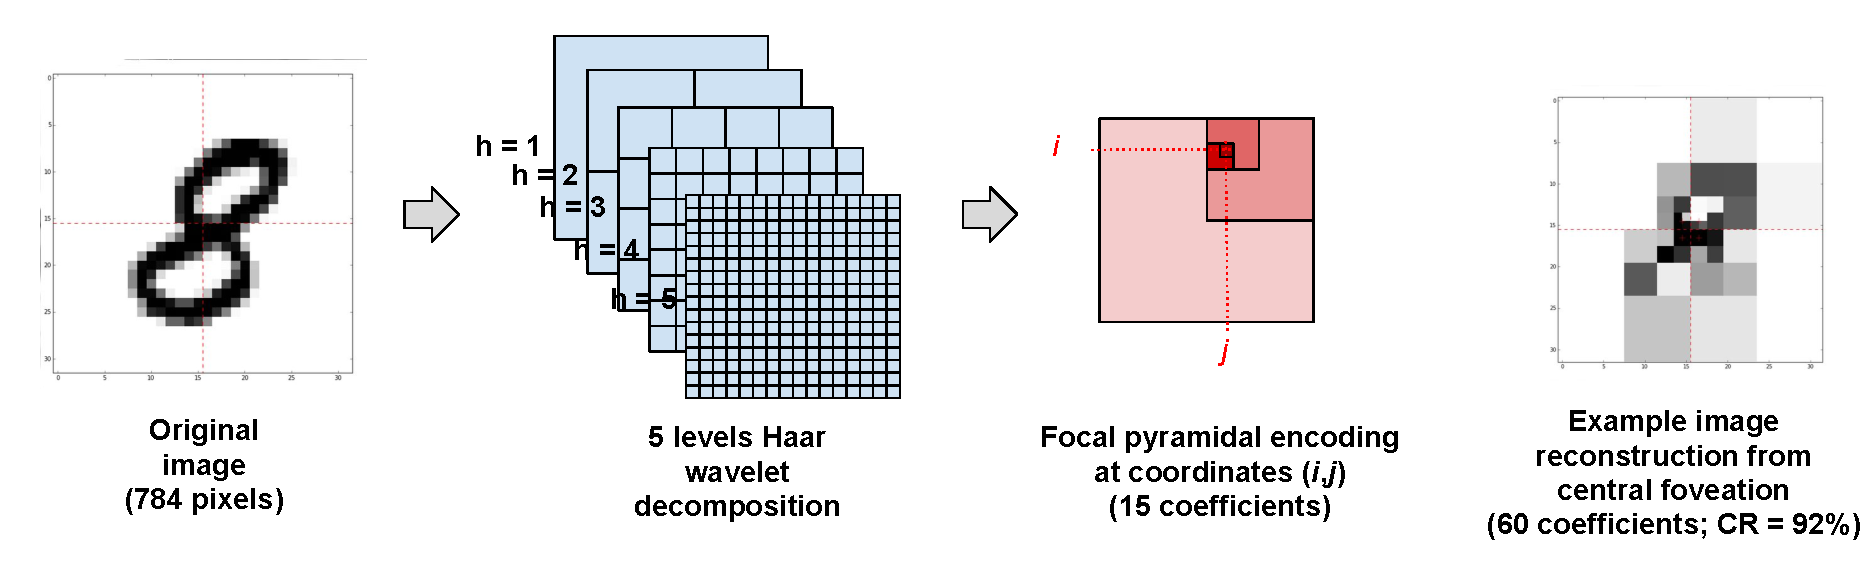
\includegraphics[width = .8\linewidth]{img/ICLR-foveated-model.pdf} 
	}
	\vspace{-.5cm}
	\caption{\textbf{a}--\textbf{c}. Foveal ``pyramidal'' encoding from image.
		\textbf{d}. Image reconstruction from 60 central coefficients, issuing a 92 \% compression rate.}\label{fig:foveated}
	\vspace{-.4cm}
\end{figure}

\begin{figure}[t]
	\vspace{0cm}
	\centerline{
	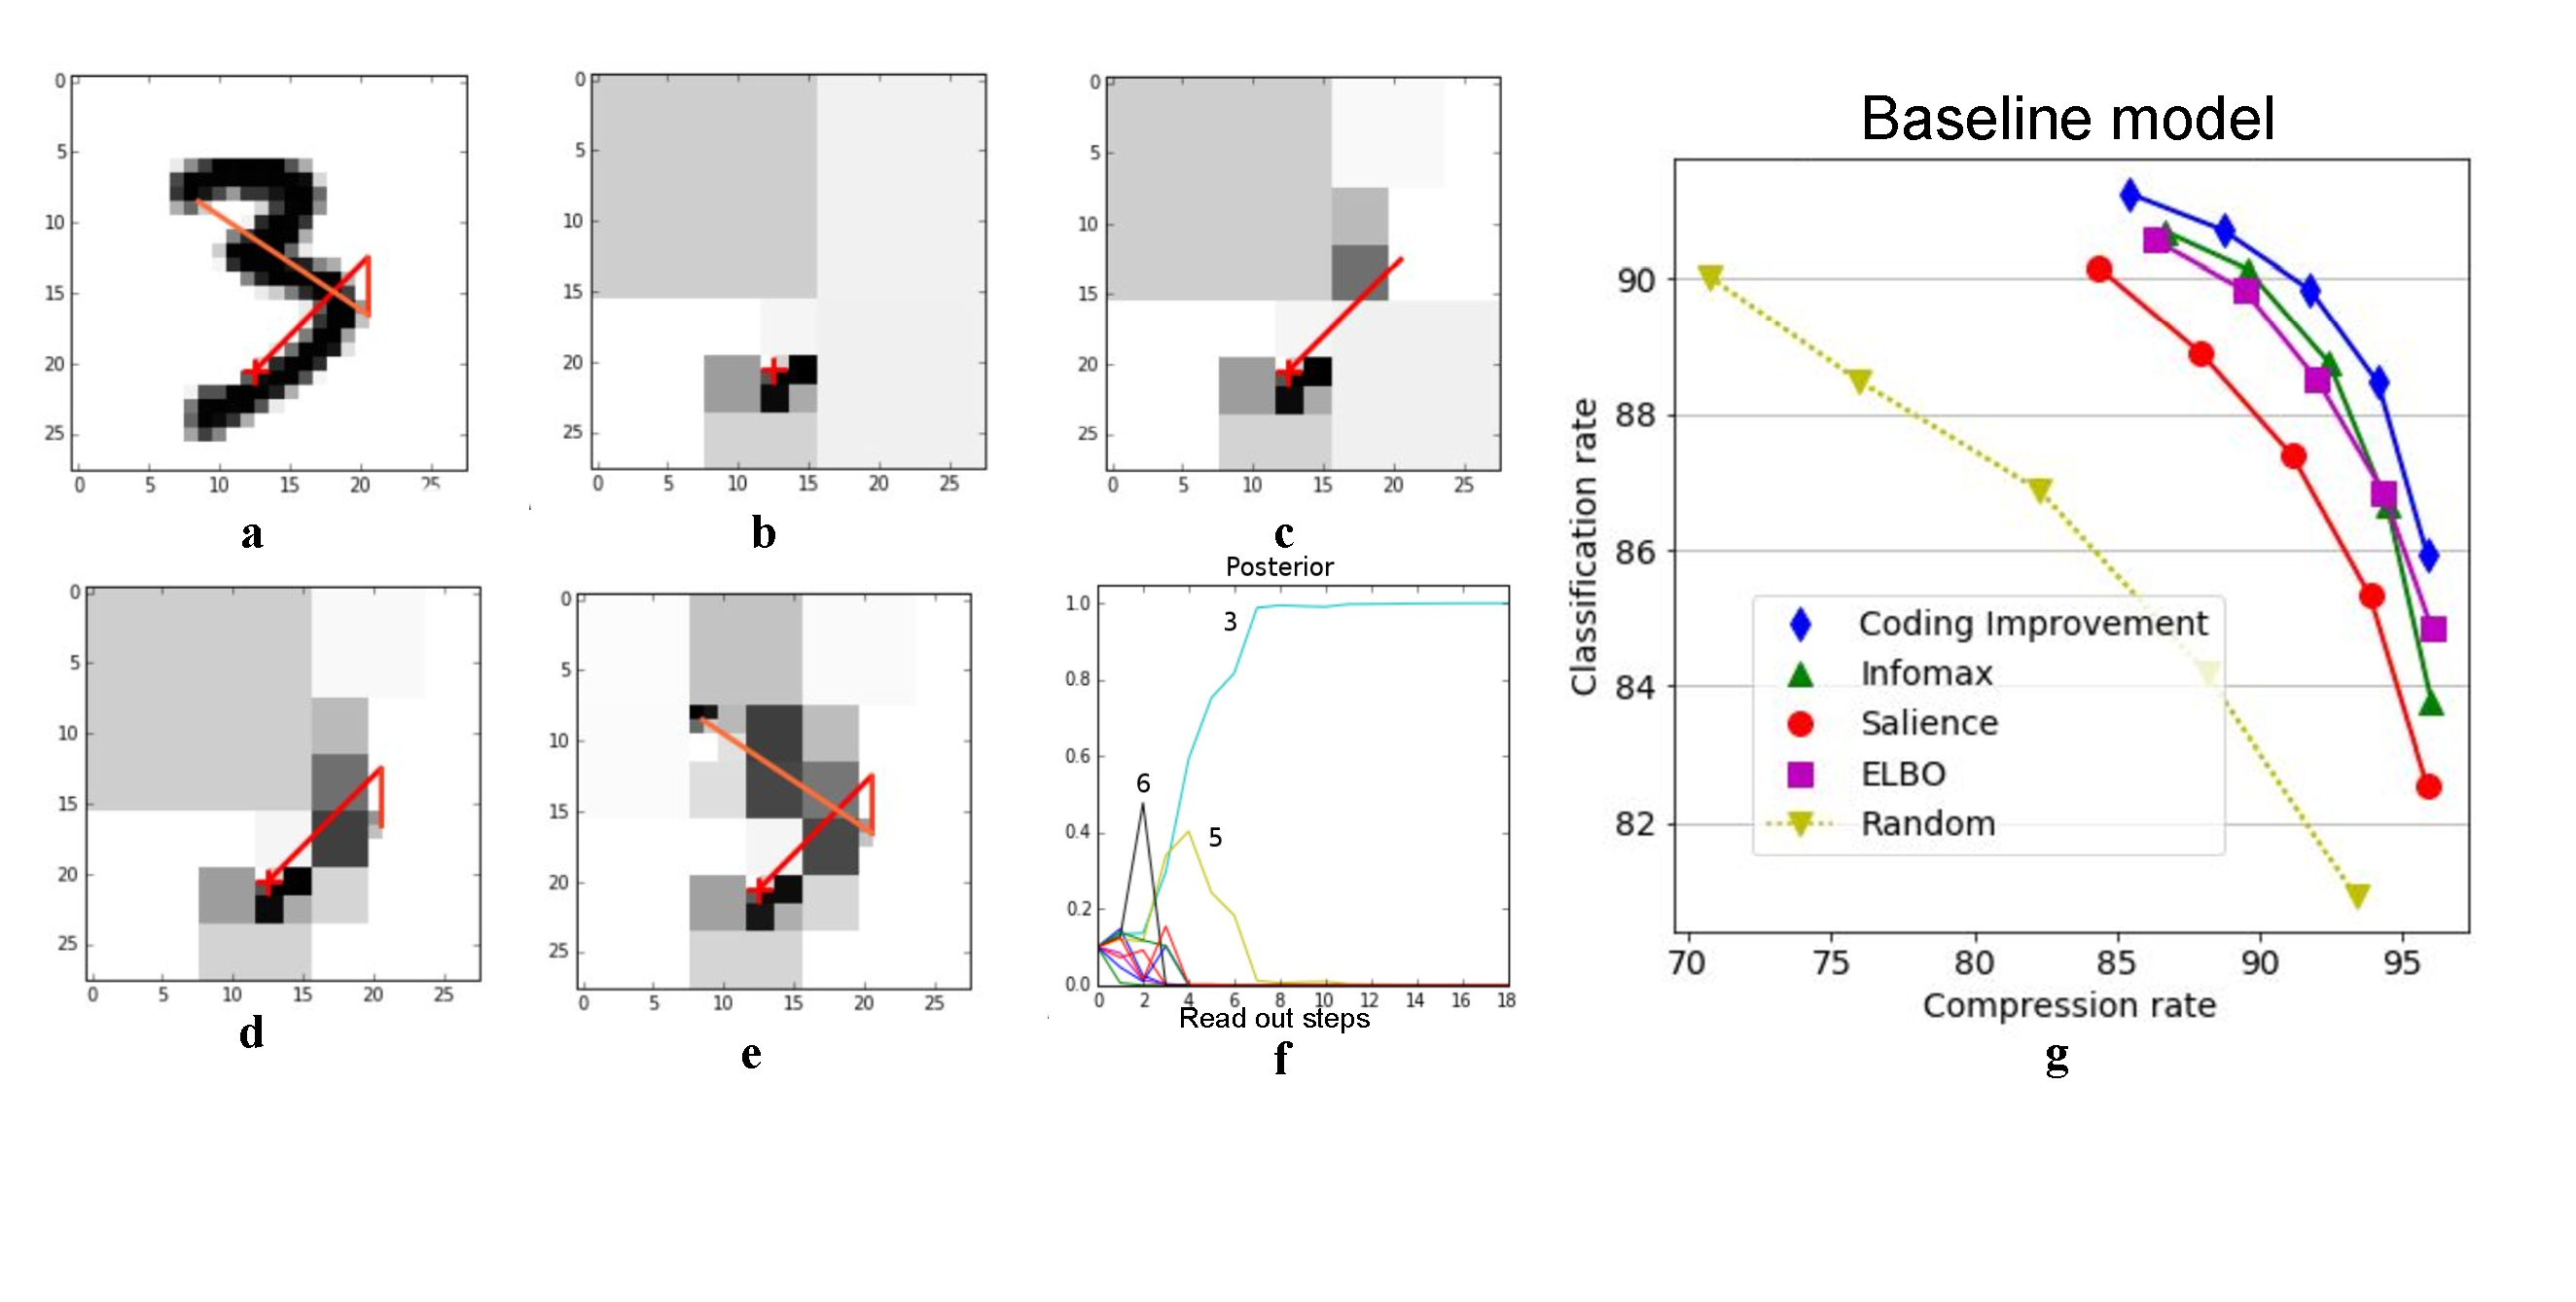
\includegraphics[width=.8\linewidth]{img/NIPS-saccade.pdf}}
	\vspace{-1.2cm}
	\caption{\textbf{Scene decoding through saccades in the foveated vision model}. \textbf{a}. Saccades trajectory over the original image (initial gaze orientation indicated with a red "plus"). \textbf{b--e}. Progressive image reconstruction over the course of saccades.
	%, with \textbf{b}: 5 coefficients triplets + root coefficient (initial gaze orientation), \textbf{c}: 9 coefficients triplets + root coefficient (first saccade), \textbf{d}: 13 coefficients triplets + root coefficient (second saccade), \textbf{e}: 17 coefficients triplets + root coefficient (third saccade) 
	\textbf{f}. Posterior update in function of the number of read-out steps.
	%(noting that step 1 stems for the root coefficient and the next steps stem for 3 Haar wavelet coefficients read-out), with one color per category (the numbers over the lines provide the competing labels) 
	\textbf{g}.  Classification rate measured on the test set in function of the decoding compression rate, for different objective functions. The stopping criterion varies from $H_\text{ref}=10^{-5}$ up to  $H_\text{ref}=10^{-1}$ (from left to right).}\label{fig:foveated-saccades}
	\vspace{-.5cm}
\end{figure}

\paragraph{Baseline generative model and decoding compression}
A generative model is learned for each $\boldsymbol{u} = (i,j,h)$ (making a total of 266 data models) over the 55,000 examples of the MNIST training set. For each category $\boldsymbol{z}$ and each gaze orientation $\boldsymbol{u}$, a generative model is built over parameter set $\Theta_{\boldsymbol{z},\boldsymbol{u}} = (\rho_{\boldsymbol{z},\boldsymbol{u}}, \boldsymbol{\mu}_{\boldsymbol{z},\boldsymbol{u}}, \boldsymbol{\Sigma}_{\boldsymbol{z},\boldsymbol{u}})$, so that 
\begin{align}
\forall \boldsymbol{z},\boldsymbol{u}, \tilde{\boldsymbol{x}}_{\boldsymbol{z},\boldsymbol{u}} \sim \mathcal{B}(\rho_{\boldsymbol{z},\boldsymbol{u}}) \times \mathcal{N}(\boldsymbol{\mu}_{\boldsymbol{z},\boldsymbol{u}}, \boldsymbol{\Sigma}_{\boldsymbol{z},\boldsymbol{u}})\label{eq:bernouilli-gated}
\end{align} 
with $\mathcal{B}$ a Bernouilli distribution and $\mathcal{N}$ a multivariate Gaussian. The role of the Bernouilli is to ``gate'' the multivariate Gaussian model in the high frequencies, where digit deformations is reflected in an alternating presence or absence of pixels for high level coefficients and at the periphery, allowing to discard the ``white'' triplets from the Gaussian moments calculation. Each resulting generative model $p(X|Z,\boldsymbol{u})$ is a mixture of Bernouilli-gated Gaussians over the 10 MNIST labels. On the encoding side, the posterior is explicitly calculated using Bayes rule, i.e. $q(Z|\boldsymbol{x},\boldsymbol{u}) = \text{softmax} \log p(\boldsymbol{x}|Z,\boldsymbol{u})$, issuing about 92\% recognition rate on the MNIST test set when combining the 266 log likelihoods of each wavelet triplet of the full images with (\ref{eq:accum}), a typical recognition rate for a shallow model.

The example of an ``Infomax''-based sequential scene decoding is presented in figure \ref{fig:foveated-saccades}\textbf{a}--\textbf{f} for one MNIST sample using algorithm \ref{algo:saccade}.
The original image is presented in fig~\ref{fig:foveated-saccades}\textbf{a} with on overlay a four ``saccades'' trajectory over the image. The corresponding decoding process is illustrated in figs~\ref{fig:foveated-saccades}\textbf{b}--\textbf{e}, giving the reconstructed pixels from  coefficients read-out at successive steps of the decoding process.
%The state of the recognition process after one saccade is shown on fig. \ref{fig:foveated-saccades}\textbf{b}. The next saccade (fig. \ref{fig:foveated-saccades}\textbf{c})  heads toward a region of the image that is expected to help confirm the guess. The continuing saccade (fig. \ref{fig:foveated-saccades}\textbf{d}) makes a close-by inspection and the final saccade (fig. \ref{fig:foveated-saccades}\textbf{e}) allows to reach the posterior entropy threshold, set at $H_\text{ref} = 1e^{-4}$ here. Fig. \ref{fig:foveated-saccades}\textbf{f} shows the posteriors update of different labels over the decoding sequence and fig. \ref{fig:foveated-saccades}\textbf{g} gives the posterior entropy update according to the coefficients triplets actually read. 
Note that several coefficient triplets are read at each end-effector position ($i,j$) (see fig. \ref{fig:foveated}c). There is for instance a total of 5 triplets read out at the initial gaze orientation (\textbf{b}), and then 4 triplets read-out for each continuing saccade. 
Last, the \emph{decoding compression rate} is defined as the proportion of wavelet coefficients that are bypassed for reaching decision. In the considered example, a total of 18 coefficient triplets is  actually read-out, representing about 7\% of the total 256 coefficient triplets, issuing a 93\% decoding compression rate. 

Fig.~\ref{fig:foveated-saccades}\textbf{g} shows the classification rate and the decoding compression rate  obtained in the test set for different objective functions and $H_\text{ref} \in \{10^{-1}, 10^{-2}, 10^{-3}, 10^{-4}, 10^{-5}\}$. The objectives are also compared with a random baseline policy. The classification rates monotonically increase with an \emph{decreasing} recognition threshold. Considering 92\% as the upper bound here, a near optimal recognition rate is obtained  at $H_\text{ref}=1e^{-5}$ for the CI objective. Though all objectives functions show a consistent increase of the classification rate with decreasing $H_\text{ref}$, the CI objective clearly overtakes the others ones. The Infomax and the ELBO behave in a close-by fashion, and then the Salience objective seems unfitted to the task. 
The compression rates are generally good, with a close to optimal classification obtained at 85\% compression. It needs to be noticed that still a correct 90\% classification rate can be obtained with random exploration at around 70\% compression rate, reflecting a strong redundancy in the original dataset.  

%The model provides apparently realistic saccades, for they cover the full range of the image and tend to point over regions that contain class-characteristic pixels. The image reconstruction after 4 saccades allows to visually recognize a "fuzzy" three, while it would not necessarily be the case if the saccades were chosen at random.
%The observed trajectory illustrates the \emph{guess confirmation} logic that is behind the active vision framework. Every saccade heads toward a region that is supposed to confirm the current hypothesis. This confirmation bias appears counter-intuitive at first sight, for some would expect the eye to head toward places that may \emph{disprove} the assumption (to challenge the current hypothesis). This is actually not the case for the class-confirming regions are more scarce than the class-disproving regions, so that heading toward a class-confirming region may bring more information in the case it would, by surprise, invalidate the initial assumption.

%{\color{green} With a final posterior approaching $1 - 1e^{-5}$, the model is actually overconfident in its own predictions which introduces a confirmation bias that may harm the final recognition rate. This is not the case in our setup (see next section for quantitative accuracy estimate), but one can not exclude the process to be overconfident at a local minimum. It must be noticed however that the confirmation bias is a more general feature of the active inference framework that should be specifically addressed (with a $T$-horizon forward planning at exponential cost and/or reward-based policy learning -- see \cite{butko2010infomax}). For there is no free lunch, it corresponds to the "price to pay" for reducing the observation range of the image at the risk of potentially neglecting critical covert information. }

\begin{figure}[b]
		\vspace{-1cm}
	\centerline{
		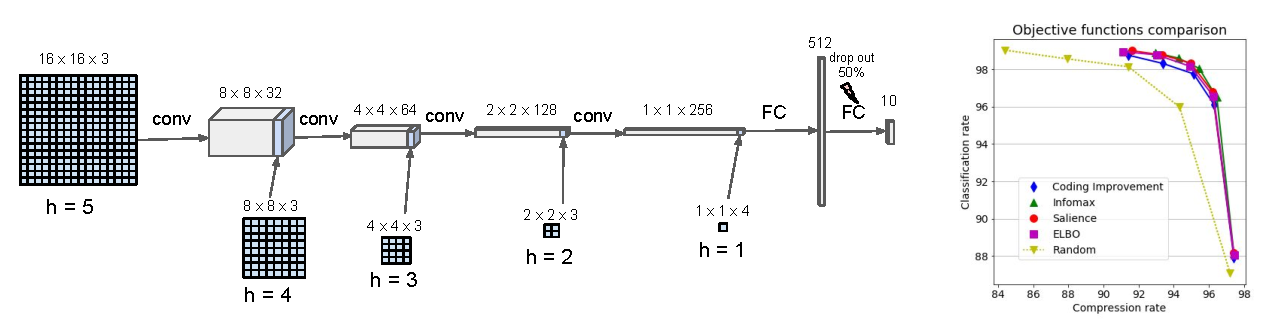
\includegraphics[width = \linewidth]{img/NIPS-convolutional.pdf} 
	}
	\vspace{-.2cm}
	\caption{\textbf{Hierarchical Convolutional Neural Network for Scene Decoding}. (Left) The CNN computational graph reflects the input hierarchical organization. (Right) Objective functions comparison on the CNN model.}\label{fig:CNN}
	\vspace{-.5cm}
\end{figure}

\begin{figure}[t]
	\vspace{-1cm}
	\centerline{
		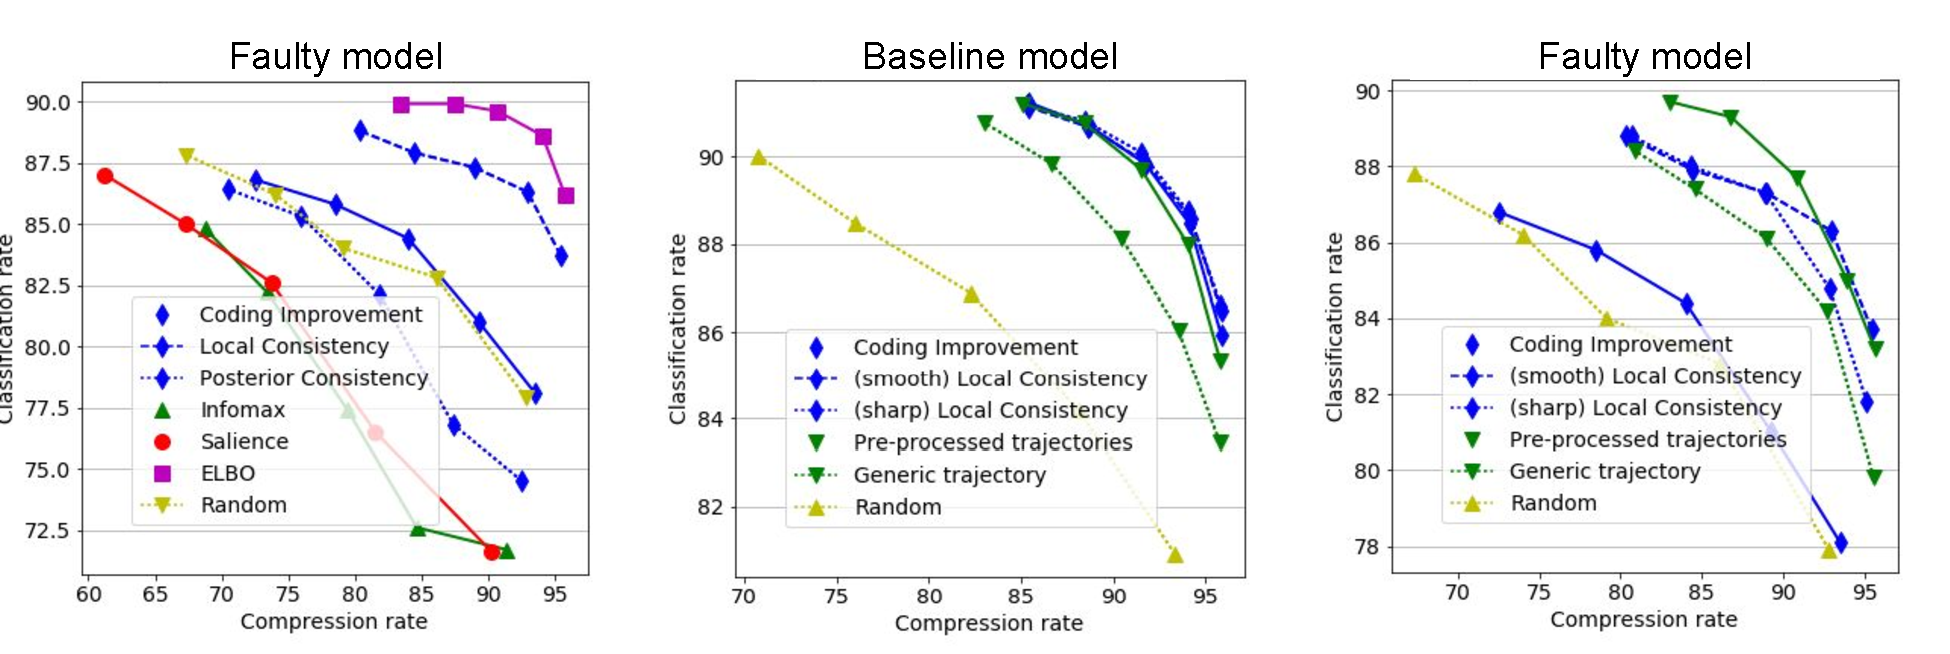
\includegraphics[width = .8\linewidth]{img/NIPS-faulty.pdf} 
	}
	\vspace{-.2cm}
	\caption{\textbf{Method comparisons}. \textbf{a}. Classification rates comparison in a faulty model (see text). \textbf{b}. Simplified computational schemes compared on the baseline shallow ``Bernoulli gated'' multivariate model. \textbf{c}. Simplified computational schemes compared on the faulty model.}\label{fig:failed}
	\vspace{-.1cm}
\end{figure}

\paragraph{Posterior update in Convolutional Neural Networks}
A convolutional neural network was designed in order to provide a more effective encoding and facilitate comparison with state-of-the-art classifiers (see fig.~\ref{fig:CNN}). 
It is made of five convolution layers having each a distinct input corresponding to the five hierarchical levels of the wavelet decomposition. 
The CNN is biasless, uses a (2,2) stride for the convolutions \emph{without max-pooling}, maximizing \emph{neighbour independence} in the convolutional computational track.
The training data was compressed at random by discarding wavelet coefficient triplets, with a varying compression rate. The network was trained during about $10^6$ epochs\footnote{trained with Tensorflow on a laptop.}. Without specific parameter tuning, the network attained a 99\% recognition rate on the test set with non-compressed wavelet transformed inputs. 
The cross-entropy loss used in training makes the network output is expected to approach the data log-likelihood, and this is how it is exploited further on. For decoding a scene, the input layers are initialized a zero  and progressively filled with new wavelet coefficients, implementing the posterior update \emph{from the data}. There is thus no recurrence, sequential accumulation or memory implemented in the network. The output is driven by adding supplementary data at the input only, complementing the data that was read out at the previous decoding steps. 
Following algorithm \ref{algo:saccade} with the CNN as the encoder, the decoding efficacy is shown for different objective functions on the right-hand side of fig.\ref{fig:CNN}. A clear decoding improvement is obtained, with higher classification rates with less signal, attaining about 98,8\% correct classification with less than 8\% of the original image. Still, the general good performances of the decoder blurs the differences between the different policies. All objectives appear here equally good at effectively decoding the scene. 

\paragraph{Faulty model and failure robustness}
The predictive policies are very dependent on the generative models and thus sensible to model flaws. Resistance to model flaws is thus a property that should be prioritized when acting in unknown or coarsely modeled environments, or in the course of learning. In contrast with CNN-based optimal decoding, we designed a failed probabilistic model by simply setting $\rho_{u,z} = 1$ in eq.~(\ref{eq:bernouilli-gated}).  This tends to overestimate the signal strength at high frequencies, predicting a dense signal in effectively sparse regions. Classification accuracies are presented on fig.~\ref{fig:failed}\textbf{a} for the different objective functions considered here. In complement to the Compression Improvement (eq.~\ref{eq:CI}), the two variants referred as the Local Consistency (eq.~\ref{eq:LC}) and the Posterior Consistency (eq.~\ref{eq:PC}) are also considered. The faulty model allows here to nicely separate the different objectives with regards to their optimistic vs. conservative flavor. While the CI stays in the middle, doing approximately as good as the random exploration, its conservative and optimistic variants respectively do better and worst than random exploration. The ELBO and the Saliency objectives, as expected, amplify this effect with a strong robustness to model flaws for the ELBO objective and, at reverse, a dramatic sensitivity  to model flaws for the 	Saliency objective. The Infomax also falls here in the optimistic category for its blindness to sequential consistency makes it update its posterior the wrong way.



\paragraph{Scaling up CI computation}
The scaling of the model needs to be addressed when large images are considered. The predictive policy relies on a mixed encoding setup that implies to consider all $\boldsymbol{u}$'s and all $\boldsymbol{z}$'s in the prediction, which scales like $O(|\mathcal{U}|\times|\mathcal{Z}|^2)$ when the predicted posterior is needed in the objective calculation, which is the case for the Infomax, the Saliency, the CI and the Posterior Consistency (algorithm \ref{algo:saccade-policy}), and $O(|\mathcal{U}|\times|\mathcal{Z}|)$ in the Local Consistency and the ELBO case for they bypass the posterior calculation. A quadratic cost may still be considered too heavy in real-case applications, implying to consider cheaper setups. A first simplification, referred as the ``sharp'' Local Consistency in  fig.~\ref{fig:failed}\textbf{b}, only samples a single $\boldsymbol{z}$ from $q^{(n-1)}$, which makes the predictive policy scale like $O(|\mathcal{U}|)$. An additional simplification can be obtained when considering the Local Consistency objective alone (eq.~\ref{eq:LC}), for it is, on contrary to all other objectives, independent of the context $q^{(n-1)}$. For a given model, all the predictive log posteriors $\log p(\boldsymbol{z}|\hat{\boldsymbol{x}}_{z,u}, \boldsymbol{u})$ can be pre-processed using the \emph{mode} of the predicted visual field $\hat{\boldsymbol{x}}_{z,u} = \underset{\boldsymbol{x}}{\text{ argmax }} p(\boldsymbol{x}|\boldsymbol{z}, \boldsymbol{u})$ as a sample, allowing, for each assumption $\boldsymbol{z}$, to \emph{pre-process} a class-specific visual exploration strategy that, given an assumption $\hat{z} = \underset{\boldsymbol{\boldsymbol{z}}}{\text{ argmax }} q^{(n)}(\boldsymbol{z})$, defines a log-posterior descending order over the $\boldsymbol{u}'s$. It is then possible to pre-process and store $|\mathcal{Z}|$ saccade trajectories of size $|\mathcal{U}|$ in a database, with a $O(|\mathcal{U}|\times|\mathcal{Z}|)$ memory load but only $\simeq O(1)$ readout computational cost. In practice, the viewpoint selected at step $n$ depends on the current guess $\hat{z}$, with on-the-fly trajectory switch if the guess is revised across the course of saccades. This strategy is referred a the \emph{pre-processed trajectories} in figs~\ref{fig:failed}\textbf{b} and \ref{fig:failed}\textbf{c}.
For comparison, a \emph{generic} trajectory was also computed using $\bar{\text{CI}}(\boldsymbol{u})
= \mathbb{E}_{\boldsymbol{z} \sim p(Z), \boldsymbol{x} \sim p(X|\boldsymbol{z}, \boldsymbol{u})}\left[ \log p(\boldsymbol{z}|\boldsymbol{x}, \boldsymbol{u})\right]$ with a uniform prior over the $\boldsymbol{z}'s$.  
It is referred a the \emph{generic trajectory} in figs~\ref{fig:failed}\textbf{b} and \ref{fig:failed}\textbf{c}.

The different simplification strategies are compared in figs~\ref{fig:failed}\textbf{b} and \ref{fig:failed}\textbf{c} over the baseline and the faulty model. Both the sharp Local Consistency and the pre-processed trajectories are shown consistent with the CI objective on fig.~\ref{fig:failed}\textbf{b}, despite their considerably lower computational cost, while the generic trajectory strategy appears less relevant. Interestingly, those computational simplifications also remain effective when robustness to model flaws is considered (fig.~\ref{fig:failed}\textbf{c}). 
Both the sharp Local Consistency and the pre-processed trajectories allow to reach both robustness and effective classification rates at lower cost.

\section{Conclusion}
A generic fovea-based scene decoding setup was presented which, accordingly with \cite{najemnik2005optimal}, rests on a predictive decoding accuracy to choose action. A variational approach to scene decoding is adopted, which, accordingly with \cite{friston2012perceptions}, optimizes the data reconstruction cost by picking new sensory samples through action. In our case, the visual field is interpreted under a \emph{mixed encoding} setup for the visual data is both generated by the viewpoint and the scene constituents. 
This allows to unify the many objective functions proposed in the literature under a single master objective referred as the Coding Improvement stated in \cite{schmidhuber2007simple}, with classical objective functions interpreted as 
approximating the CI in either a conservative or an optimistic fashion. The numerical experiments proposed in the following thus highlight different aspects of the setup. 
A first and principal result is that state-of-the-art recognition rate can be obtained with sequential fovea-based computation using less than 10\% of the original signal. This strong input compression is rendered possible for the visual data owns lot of redundancies that are not used at their best, doing useless computations over large parts of the visual scene. A second result is the sub-optimality of many classical objective function widely used in literature, like the ``Infomax'' \citep{butko2010infomax} and the ``Salience'' objectives \citep{itti2005bayesian}. Their sub-optimality is not manifest with finely-tuned generative models, but become visible when a coarse of faulty model is used.  
Last, a variant of the CI objective, named the Local Consistency, is shown to provide both a good robustness to model flaws and ways toward cheap and scalable predictive policies.  


%\section*{References}
\bibliographystyle{apalike}
\bibliography{biblio}



\end{document}
